% this TeX file provides an awesome example of how TeX will make super 
% awesome tables, at the cost of your of what happens when you try to make a
% table that is very complicated.
\documentclass[11pt]{article}

% Use wide margins, but not quite so wide as fullpage.sty
\marginparwidth 0.5in 
\oddsidemargin 0.25in 
\evensidemargin 0.25in 
\marginparsep 0.25in
\topmargin 0.25in
\textwidth 6in
\textheight 8in
% That's about enough definitions

% language input
\usepackage[utf8]{inputenc}
% multirow allows you to combine rows in columns
\usepackage{multirow}
% tabularx allows manual tweaking of column width
\usepackage{tabularx}
% insert images
\usepackage{graphicx}
\usepackage{float}
\graphicspath{ {images/} }

\begin{document}
% this is an alternate method of creating a title
%\hfill\vbox{\hbox{Gius, Mark}
%       \hbox{Cpe 456, Section 01}  
%       \hbox{Lab 1}    
%       \hbox{\today}}\par
%
%\bigskip
%\bigskip
\author{Vandré Leal Cândido}
\title{Wireshark Lab: DNS v6.01}
\maketitle

% 1. nslookup
\section{nslookup}

%\begin{figure}[H]
%\centering
%\caption{Request (Section 1)}
%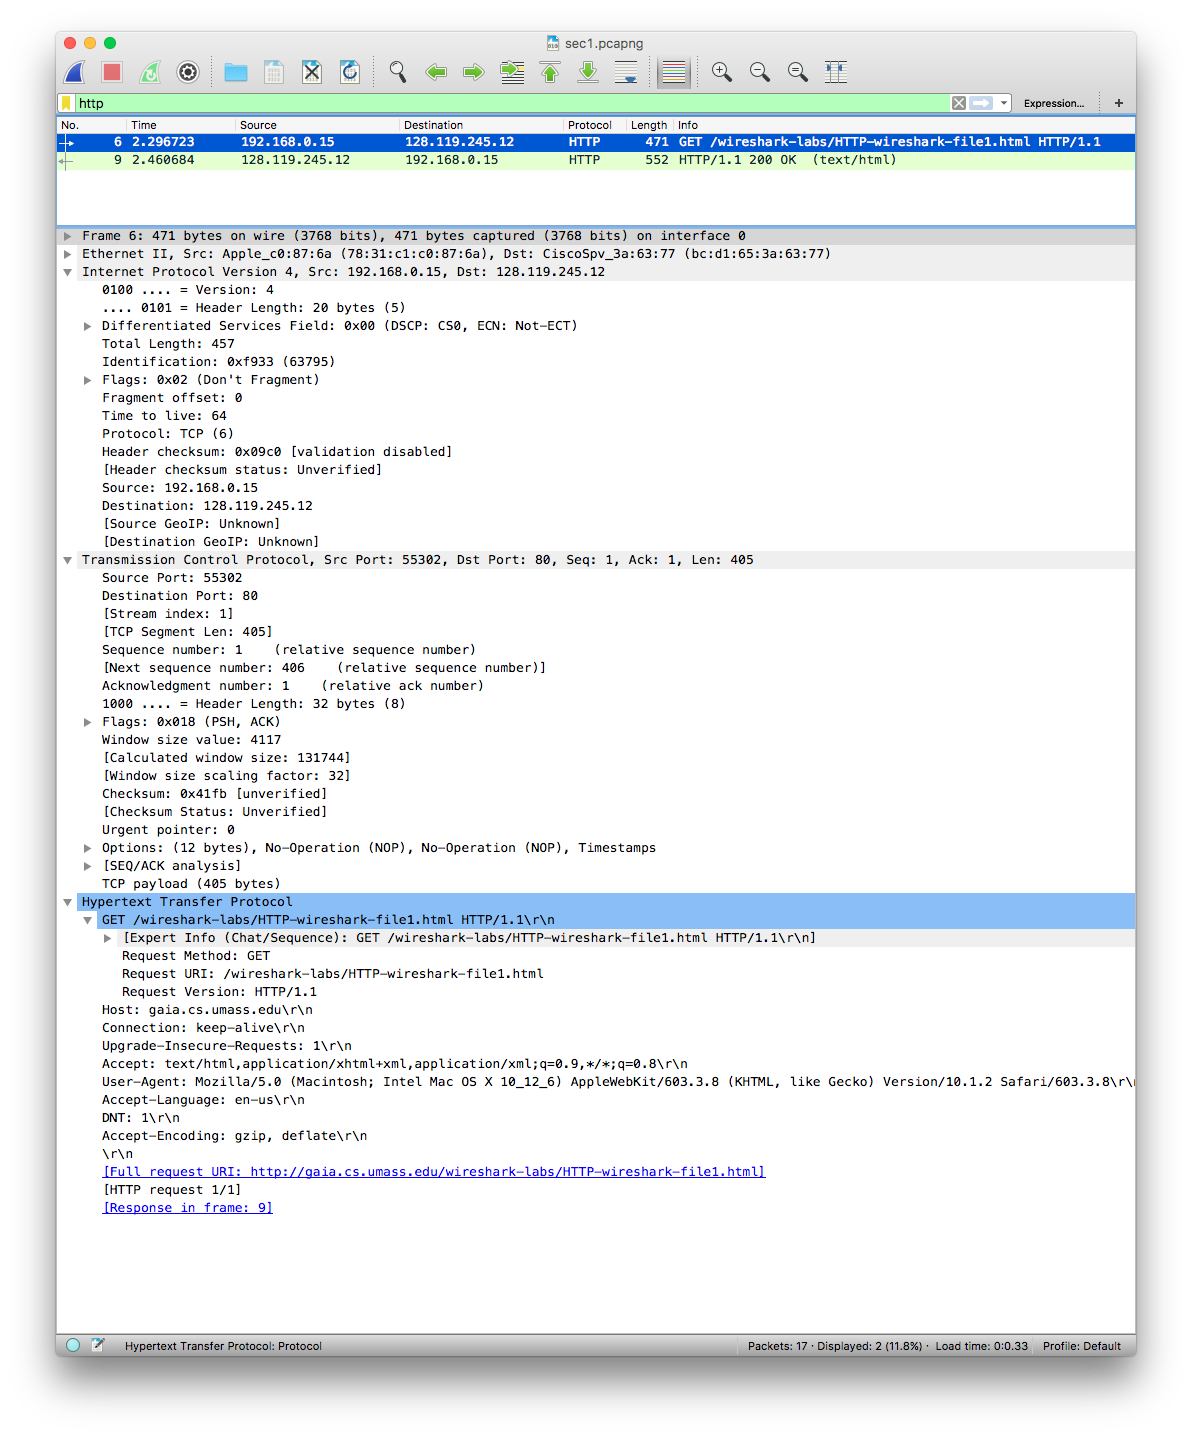
\includegraphics[width=\textwidth]{01-request}
%\end{figure}

\begin{itemize}
	\setlength\itemsep{.5cm}

	\item
		\textit{Run nslookup to obtain the IP address of a Web server in Asia. What is the IP address of that server?}
		\par The IP address is 133.11.7.85
		
		\begin{figure}[H]
		\centering
		\caption{Question 01}
		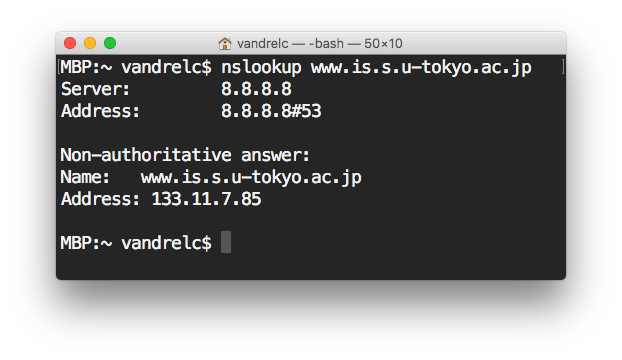
\includegraphics[width=350px]{01}
		\end{figure}
	
	\pagebreak
	
	\item
		\textit{Run nslookup to determine the authoritative DNS servers for a university in Europe.}
		\par The authoritative DNS server is reld01.insa-rennes.fr.
		
		\begin{figure}[H]
		\centering
		\caption{Question 02}
		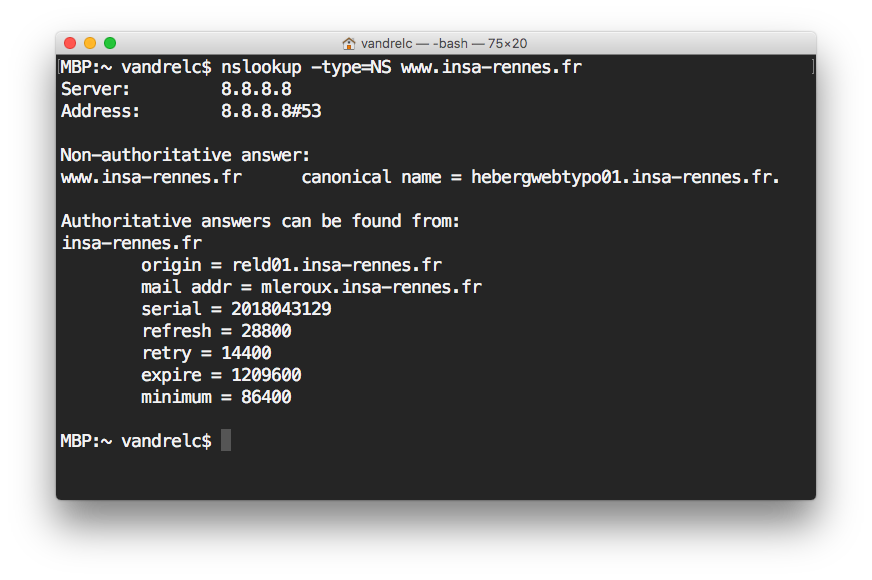
\includegraphics[width=375px]{02}
		\end{figure}
	
	\item
		\textit{Run nslookup so that one of the DNS servers obtained in Question 2 is queried for the mail
servers for Yahoo! mail. What is its IP address?}
		\par The IP address is 193.52.94.2.
		
		\begin{figure}[H]
		\centering
		\caption{Question 03}
		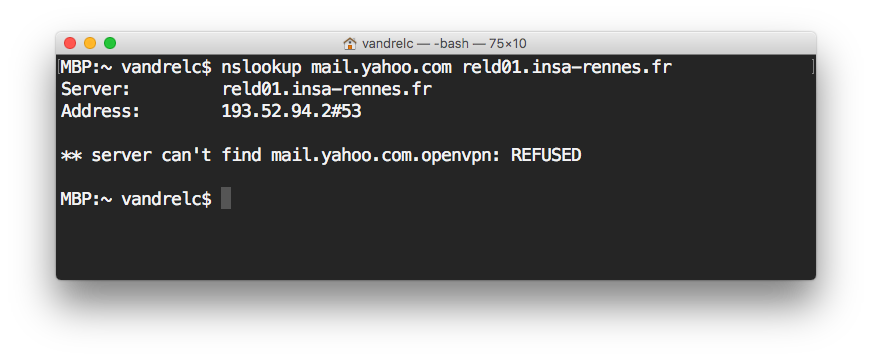
\includegraphics[width=375px]{03}
		\end{figure}
	
\end{itemize}

% 3. Tracing DNS with Wireshark
\section{Tracing DNS with Wireshark}

		\begin{figure}[H]
		\centering
		\caption{DNS Query Message}
		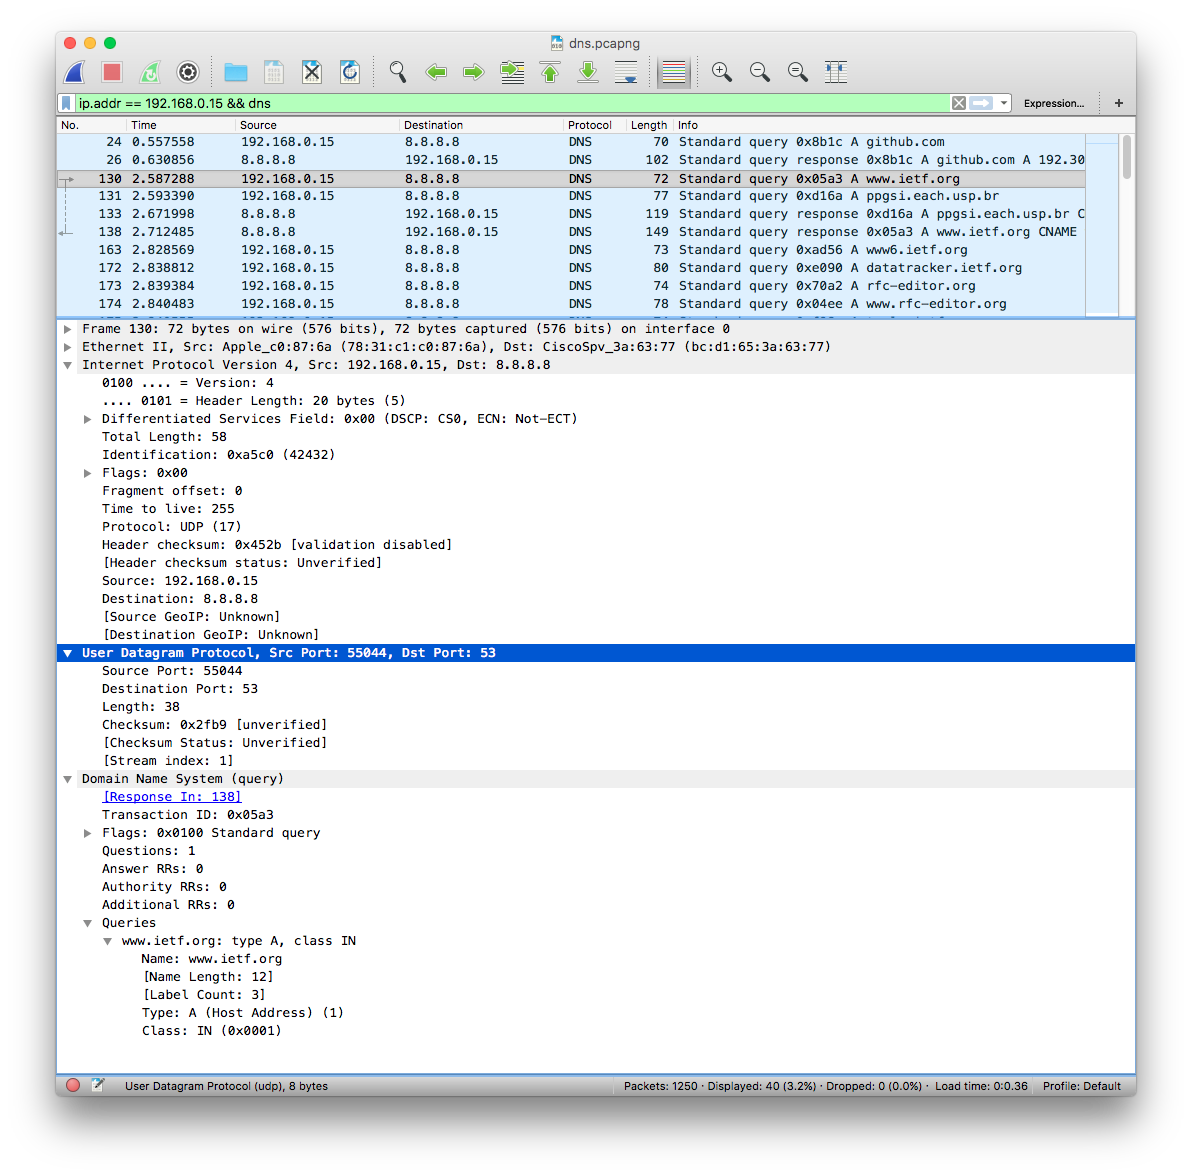
\includegraphics[width=460px]{04}
		\end{figure}
		
		\begin{figure}[H]
		\centering
		\caption{DNS Response Message}
		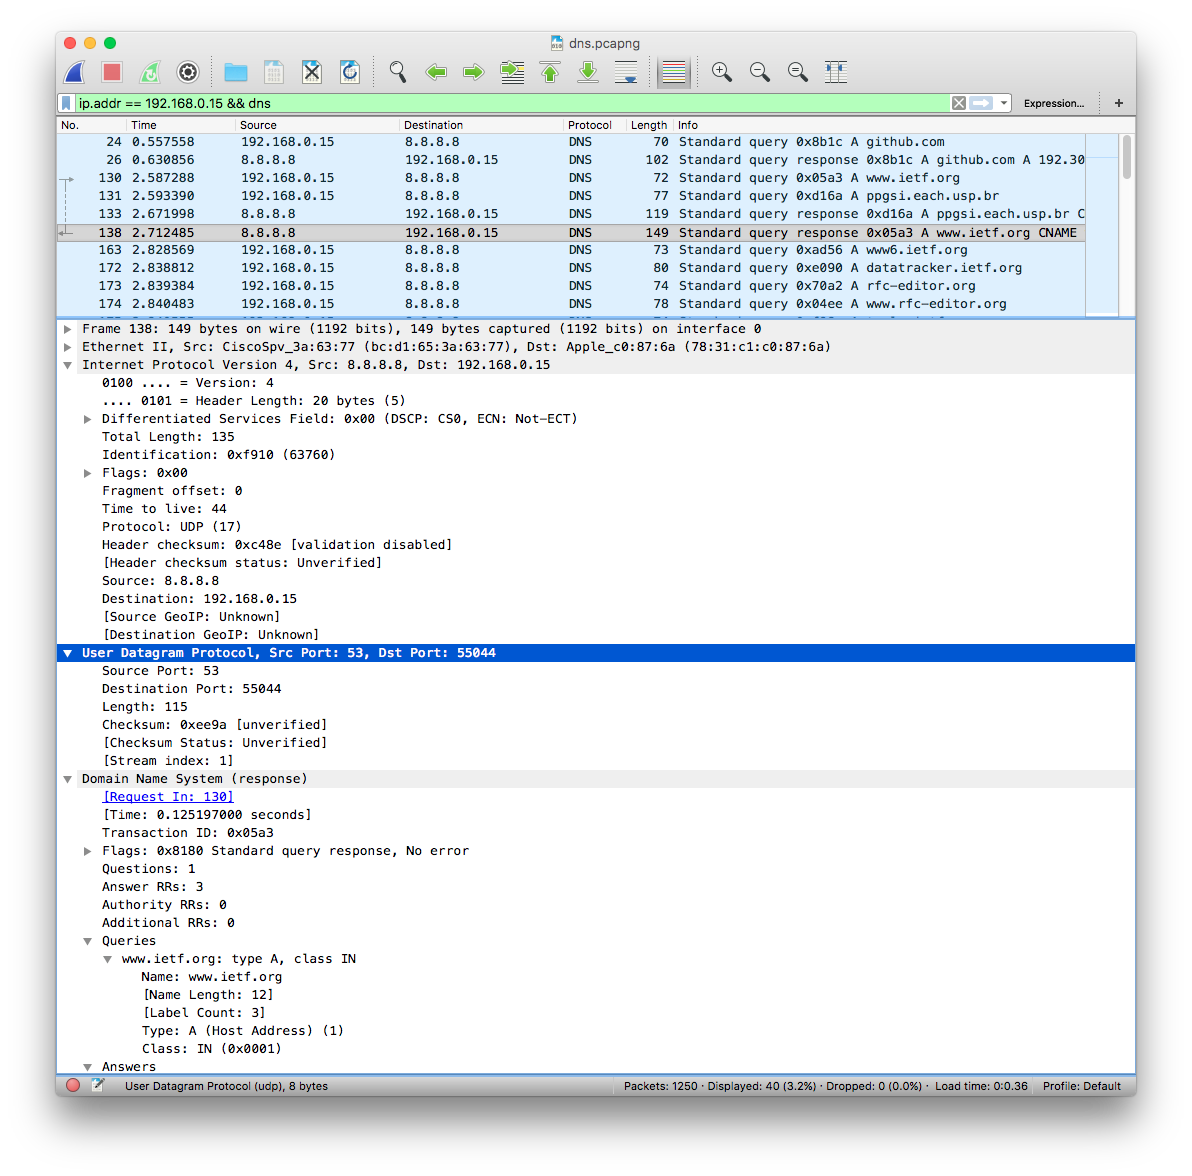
\includegraphics[width=460px]{05}
		\end{figure}
		
\pagebreak
		
\begin{itemize}
	\setlength\itemsep{.5cm}

	\item
		\textit{Locate the DNS query and response messages. Are then sent over UDP or TCP?}
		\par Both the query and response messages are sent over UDP.

	\item
		\textit{What is the destination port for the DNS query message? What is the source port of DNS
response message?}
		\par The destination port of the DNS query message is 53. The source port of the response message is also 53.
		
	\item
		\textit{To what IP address is the DNS query message sent? Use ipconfig to determine the IP address
of your local DNS server. Are these two IP addresses the same?}
		\par The DNS query message is sent to 8.8.8.8, which is the IP address of one of the local DNS servers (Google DNS).
		
		\begin{figure}[H]
		\centering
		\caption{Local DNS servers}
		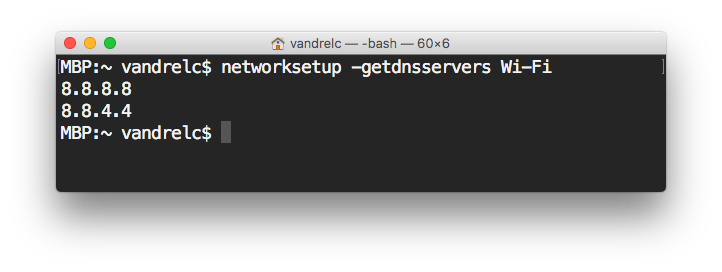
\includegraphics[width=350px]{06}
		\end{figure}
		
	\item
		\textit{Examine the DNS query message. What “Type” of DNS query is it? Does the query message
contain any “answers”?}
		\par It's a standard query (Type A). It doesn't contain any answers.

	\item
		\textit{Examine the DNS response message. How many “answers” are provided? What do each of
these answers contain?}
		\par 3 answers were provided. Each answer contains the following information: name of the host, type, class, TTL, data length and IP address.
		
		\begin{figure}[H]
		\centering
		\caption{DNS response answers}
		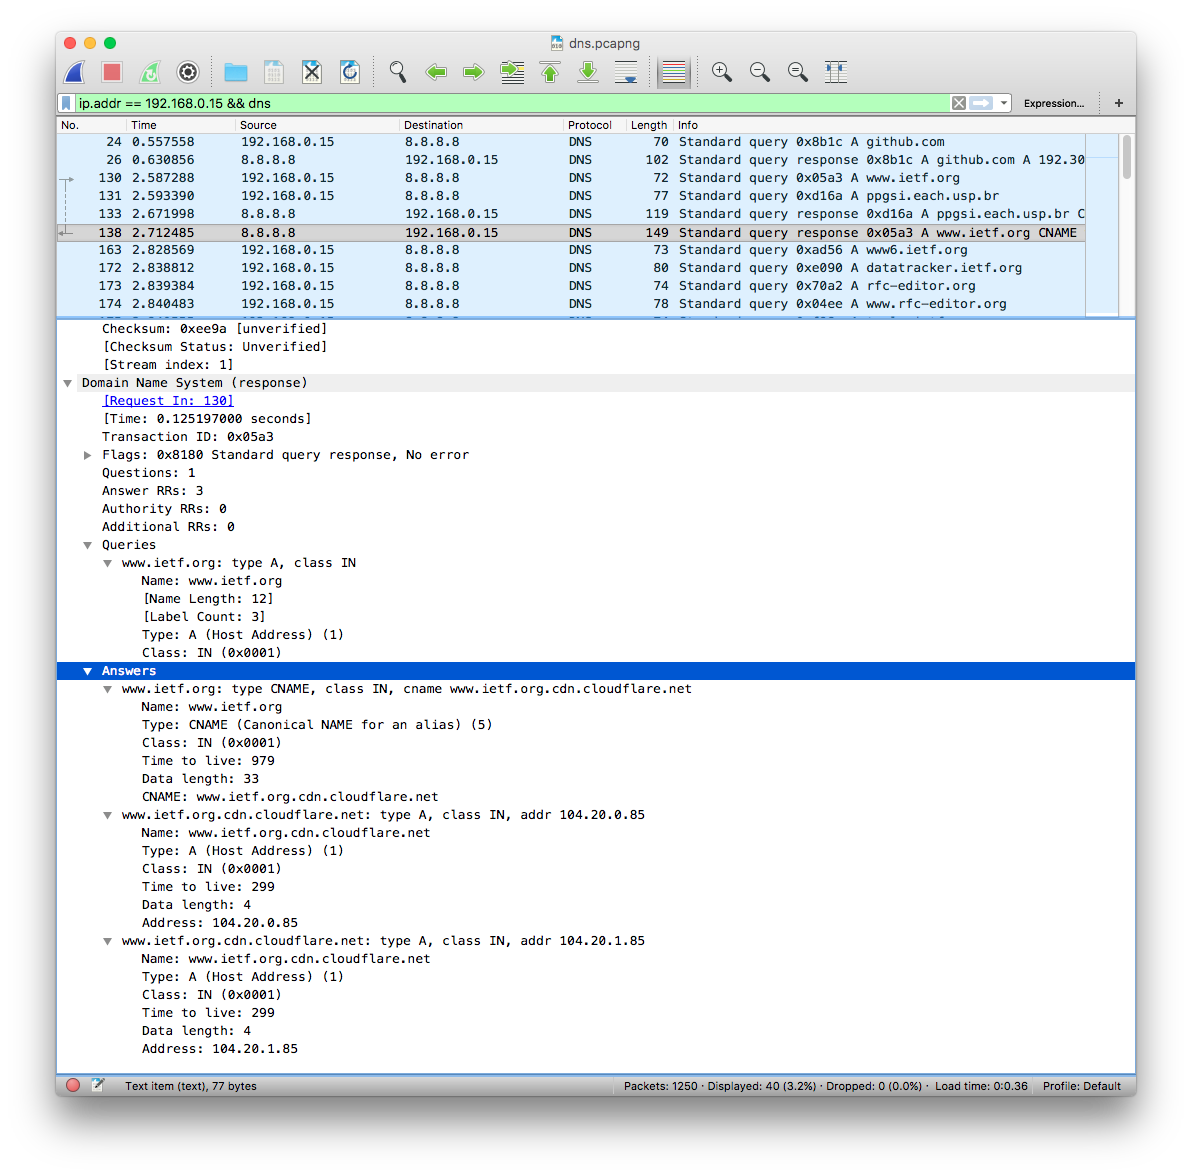
\includegraphics[width=460px]{07}
		\end{figure}
		
	\item
		\textit{Consider the subsequent TCP SYN packet sent by your host. Does the destination IP address of the SYN packet correspond to any of the IP addresses provided in the DNS response message?}
		\par Yes, the first SYN packet was sent to 104.20.0.85 which is one of the IP addresses provided in the DNS response message.
		
		\begin{figure}[H]
		\centering
		\caption{TCP SYN packet}
		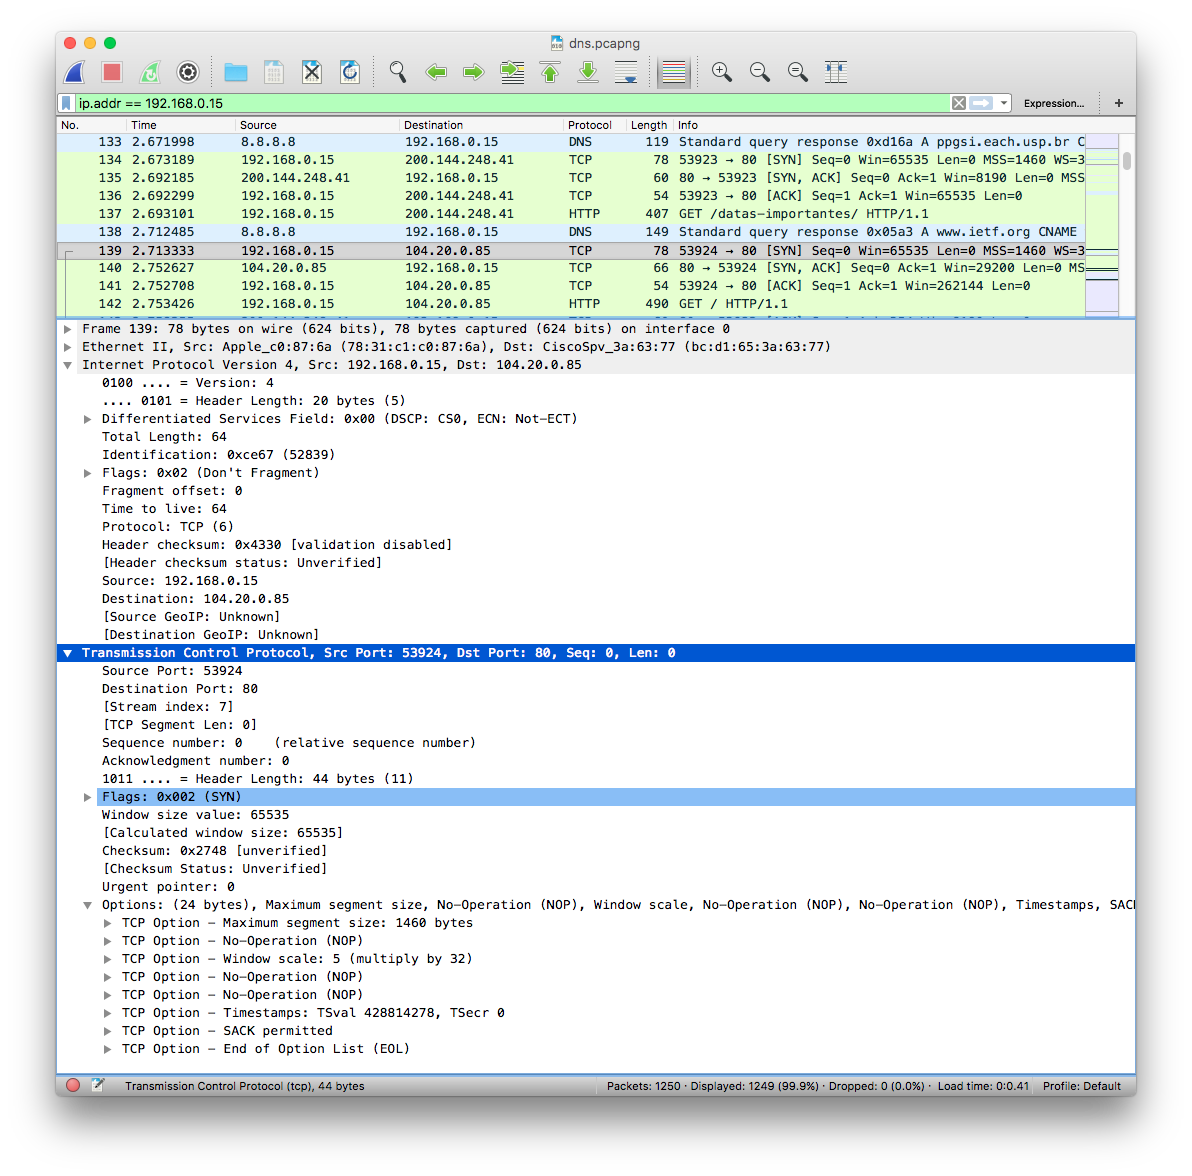
\includegraphics[width=460px]{08}
		\end{figure}

	\item
		\textit{This web page contains images. Before retrieving each image, does your host issue new DNS queries?}
		\par No.
		
\pagebreak

\par Now let’s play with nslookup.
\begin{itemize}
	\item Start packet capture.
	\item Do an nslookup on www.mit.edu
	\item Stop packet capture.
\end{itemize}

		\begin{figure}[H]
		\centering
		\caption{nslookup www.mit.edu (DNS Request)}
		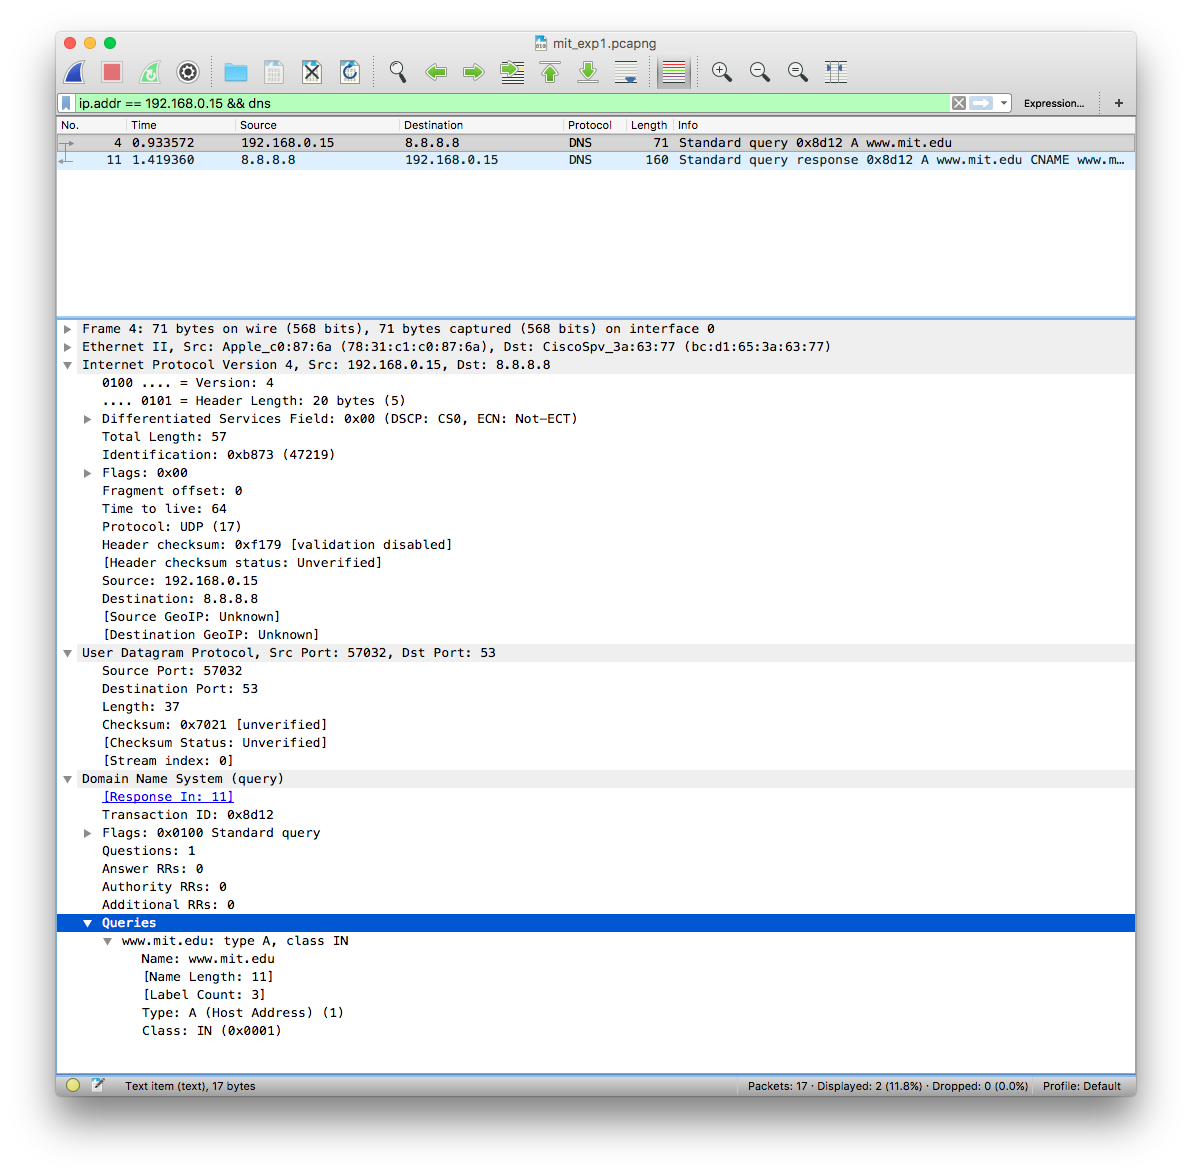
\includegraphics[width=400px]{09}
		\end{figure}
		
		\begin{figure}[H]
		\centering
		\caption{nslookup www.mit.edu (DNS Response)}
		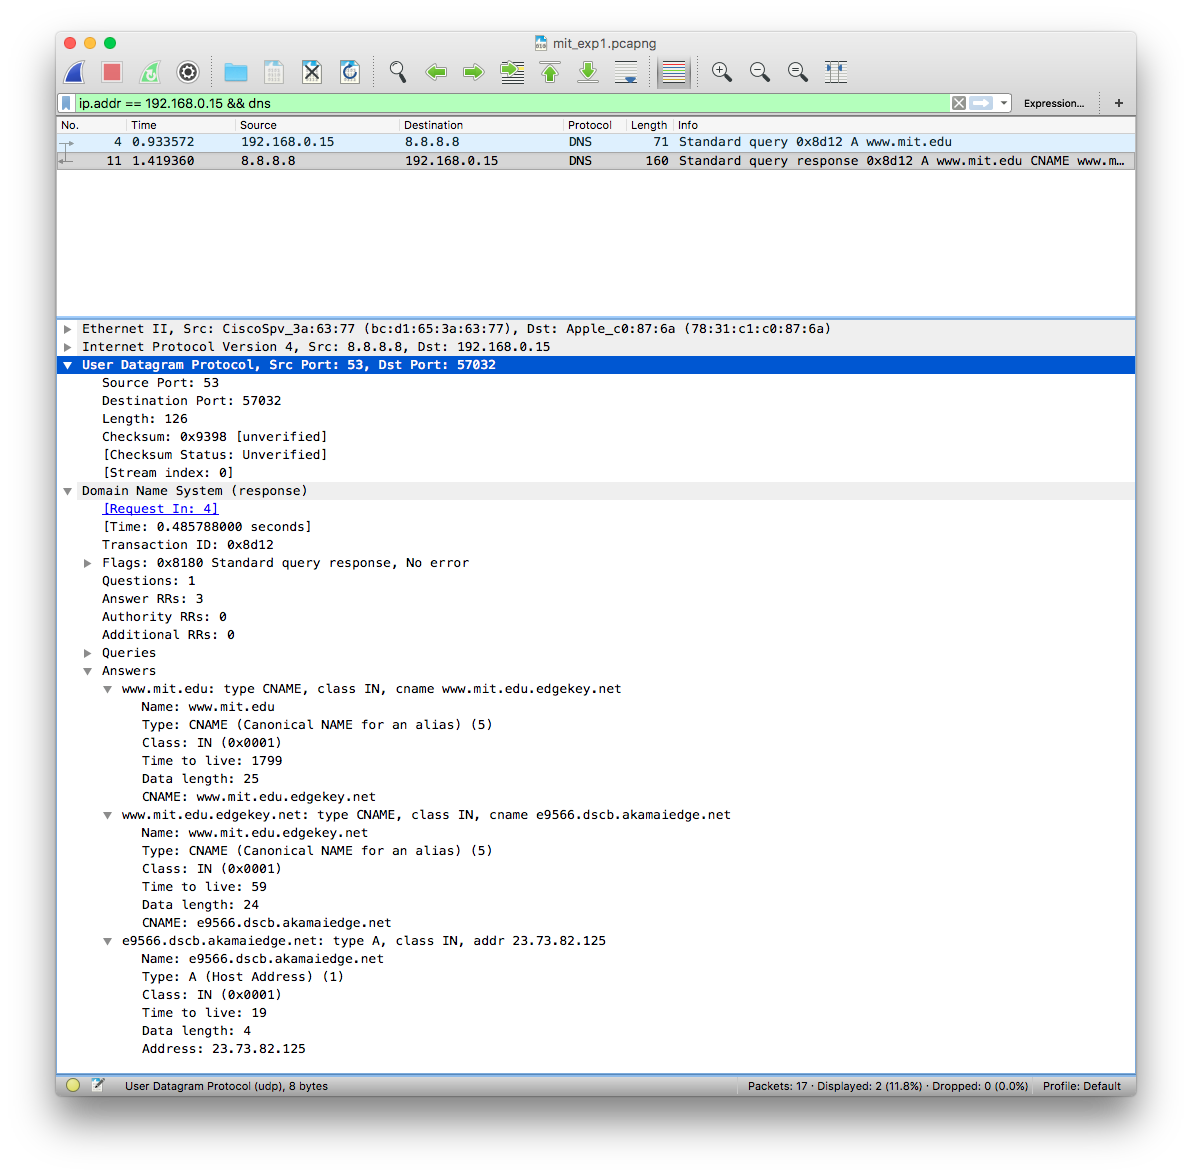
\includegraphics[width=400px]{10}
		\end{figure}

	\item
		\textit{What is the destination port for the DNS query message? What is the source port of DNS response message?}
		\par The destination port of the DNS query message is 53. The source port of the response message is also 53.
		
	\item
		\textit{To what IP address is the DNS query message sent? Is this the IP address of your default local DNS server?}
		\par The DNS query message is sent to 8.8.8.8, which is the IP address of one of the local DNS servers.
		
	\item
		\textit{Examine the DNS query message. What “Type” of DNS query is it? Does the query message contain any “answers”?}
		\par Type A. It doesn't contain any answers.
		
	\item
		\textit{Provide a screenshot.}
		\par Figure \ref{fig:11}.
		
		\begin{figure}[H]
		\centering
		\caption{nslookup www.mit.edu (DNS Response Answers)}
		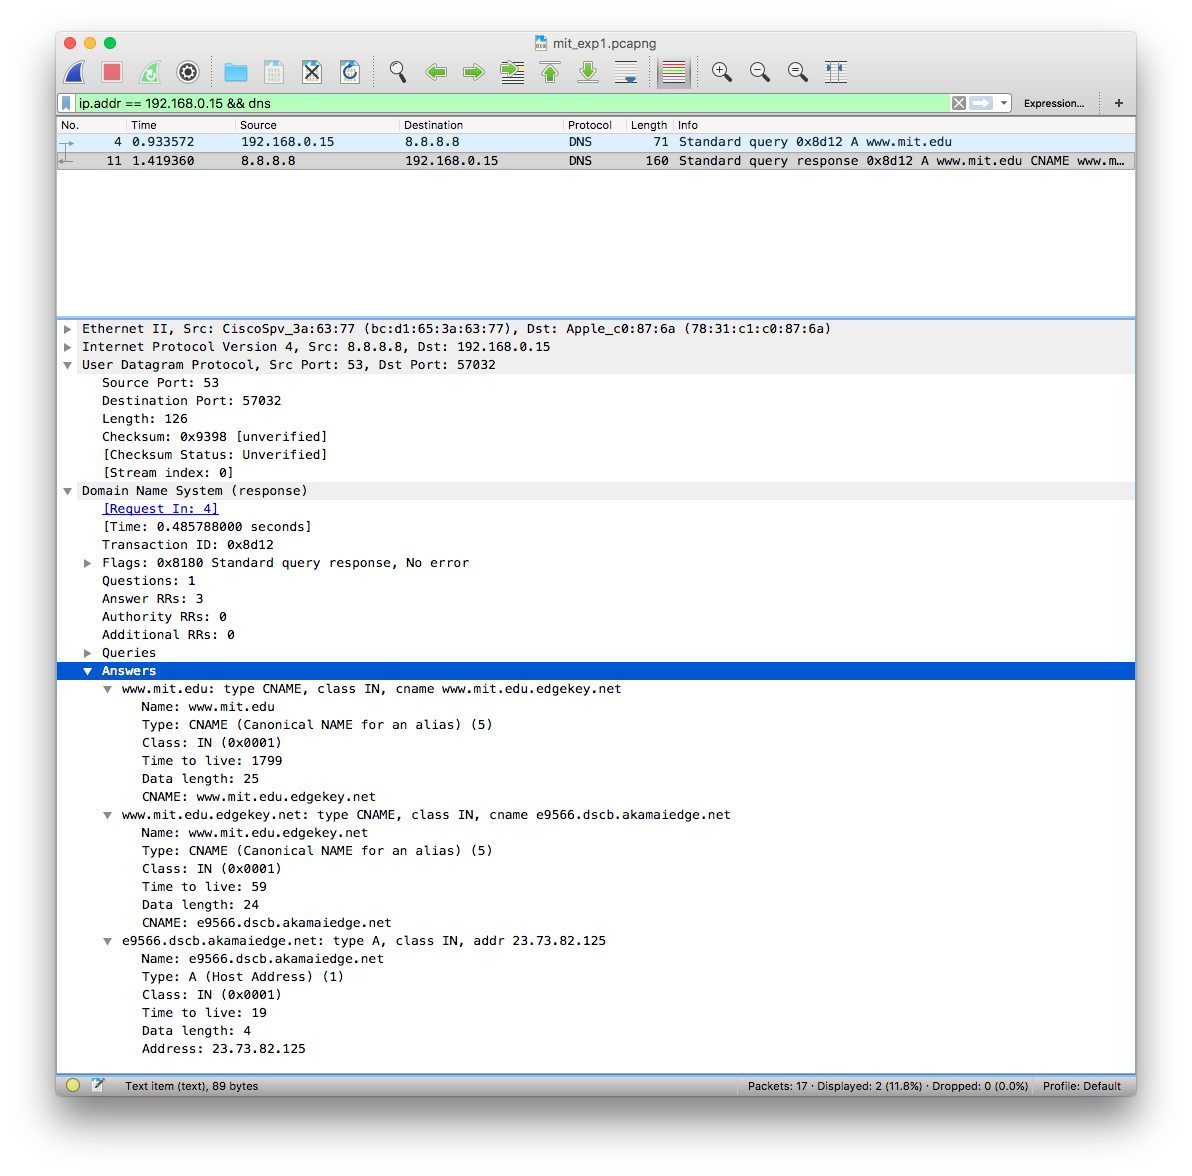
\includegraphics[width=400px]{11}
		\label{fig:11}
		\end{figure}
		
\pagebreak

\par Now repeat the previous experiment, but instead issue the command:
\par nslookup –type=NS mit.edu

		\begin{figure}[H]
		\centering
		\caption{nslookup –type=NS mit.edu (DNS Request)}
		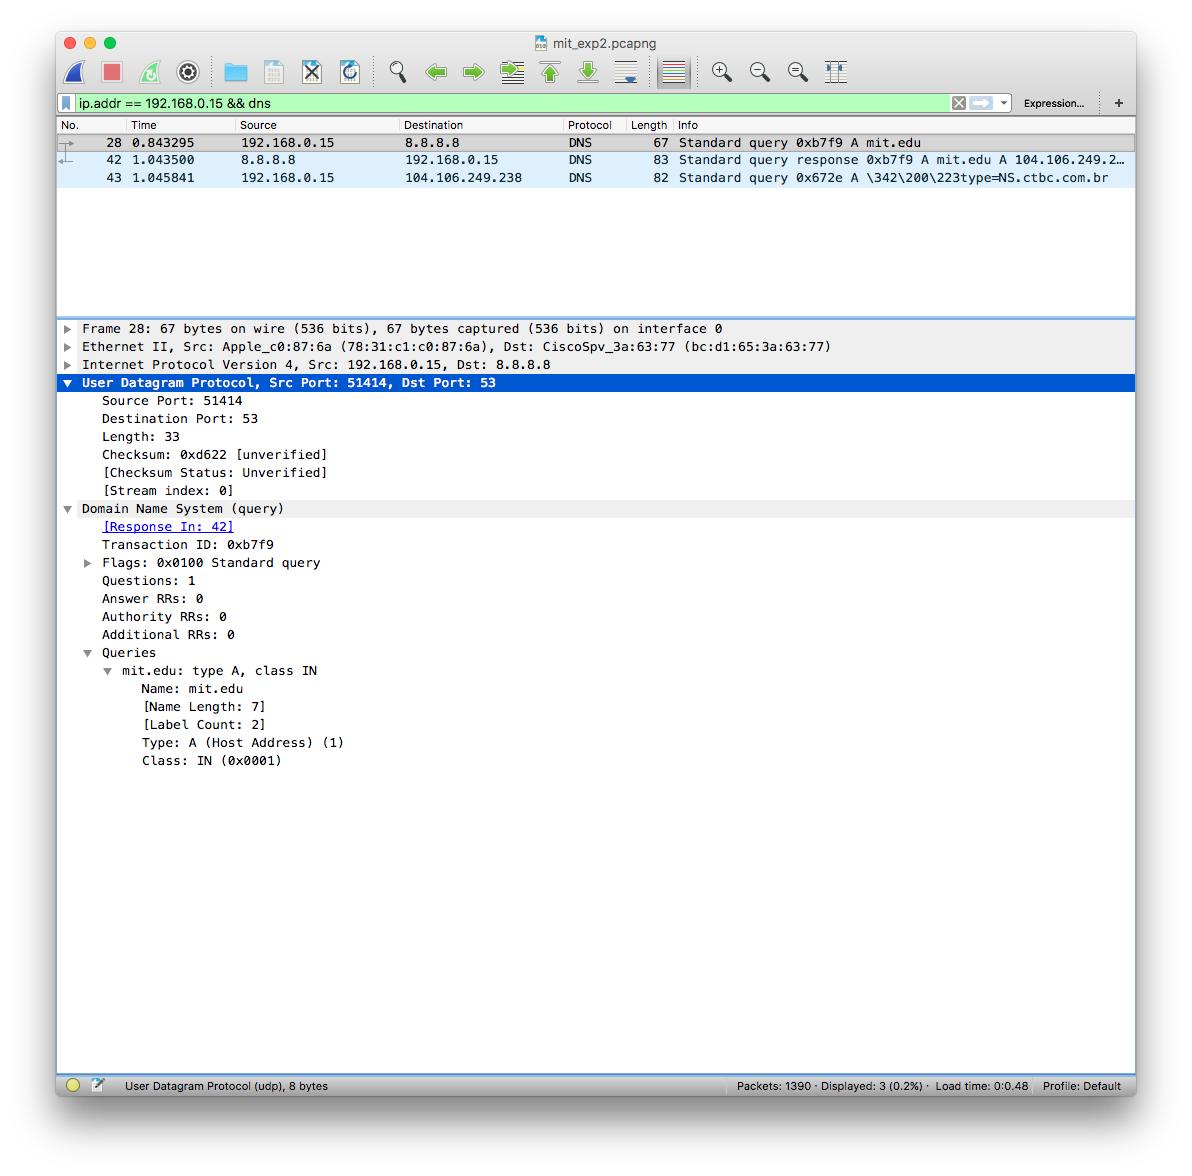
\includegraphics[width=460px]{12}
		\label{fig:12}
		\end{figure}
		
		\begin{figure}[H]
		\centering
		\caption{nslookup –type=NS mit.edu (DNS Response)}
		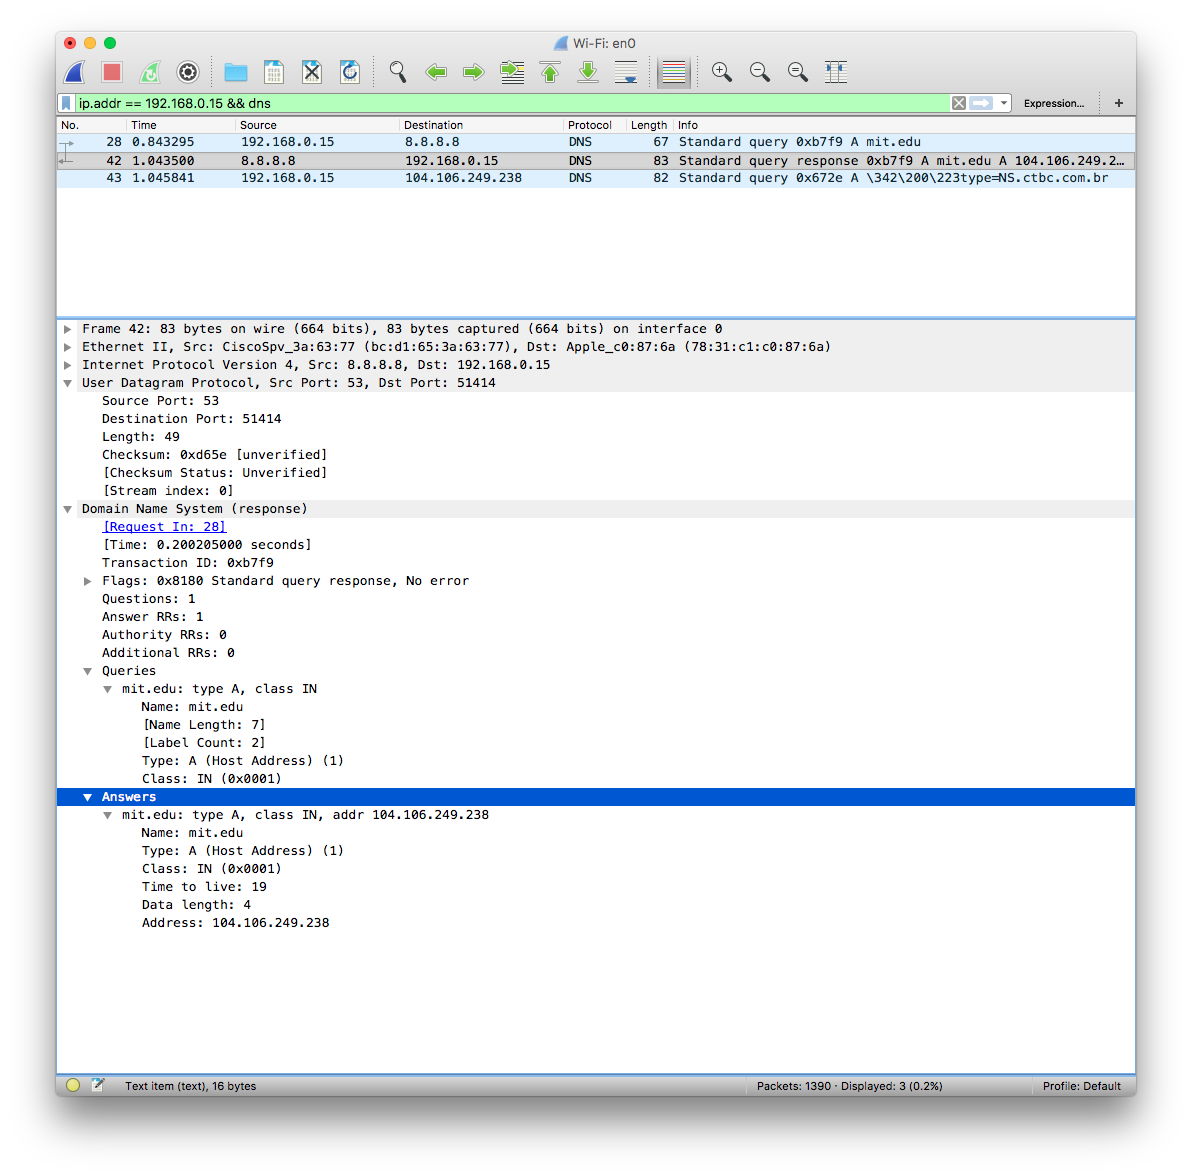
\includegraphics[width=460px]{13}
		\label{fig:13}
		\end{figure}
		
\pagebreak

	\item
		\textit{To what IP address is the DNS query message sent? Is this the IP address of your default local DNS server?}
		\par The DNS query message is sent to 8.8.8.8, which is the IP address of one of the local DNS servers.
		
	\item
		\textit{Examine the DNS query message. What “Type” of DNS query is it? Does the query message contain any “answers”?}
		\par Type A. It doesn't contain any answers.
		
	\item
		\textit{Examine the DNS response message. What MIT nameservers does the response message provide? Does this response message also provide the IP addresses of the MIT nameservers?}
		\par The message provides an unique answer that provides info for the server name `mit.edu' which address is 104.106.249.238.
		
	\item
		\textit{Provide a screenshot.}
		\par Figures \ref{fig:12} and \ref{fig:13}.
		
\pagebreak

\par Now repeat the previous experiment, but instead issue the command:
\par nslookup www.aiit.or.kr bitsy.mit.edu

		\begin{figure}[H]
		\centering
		\caption{nslookup www.aiit.or.kr bitsy.mit.edu (DNS Request)}
		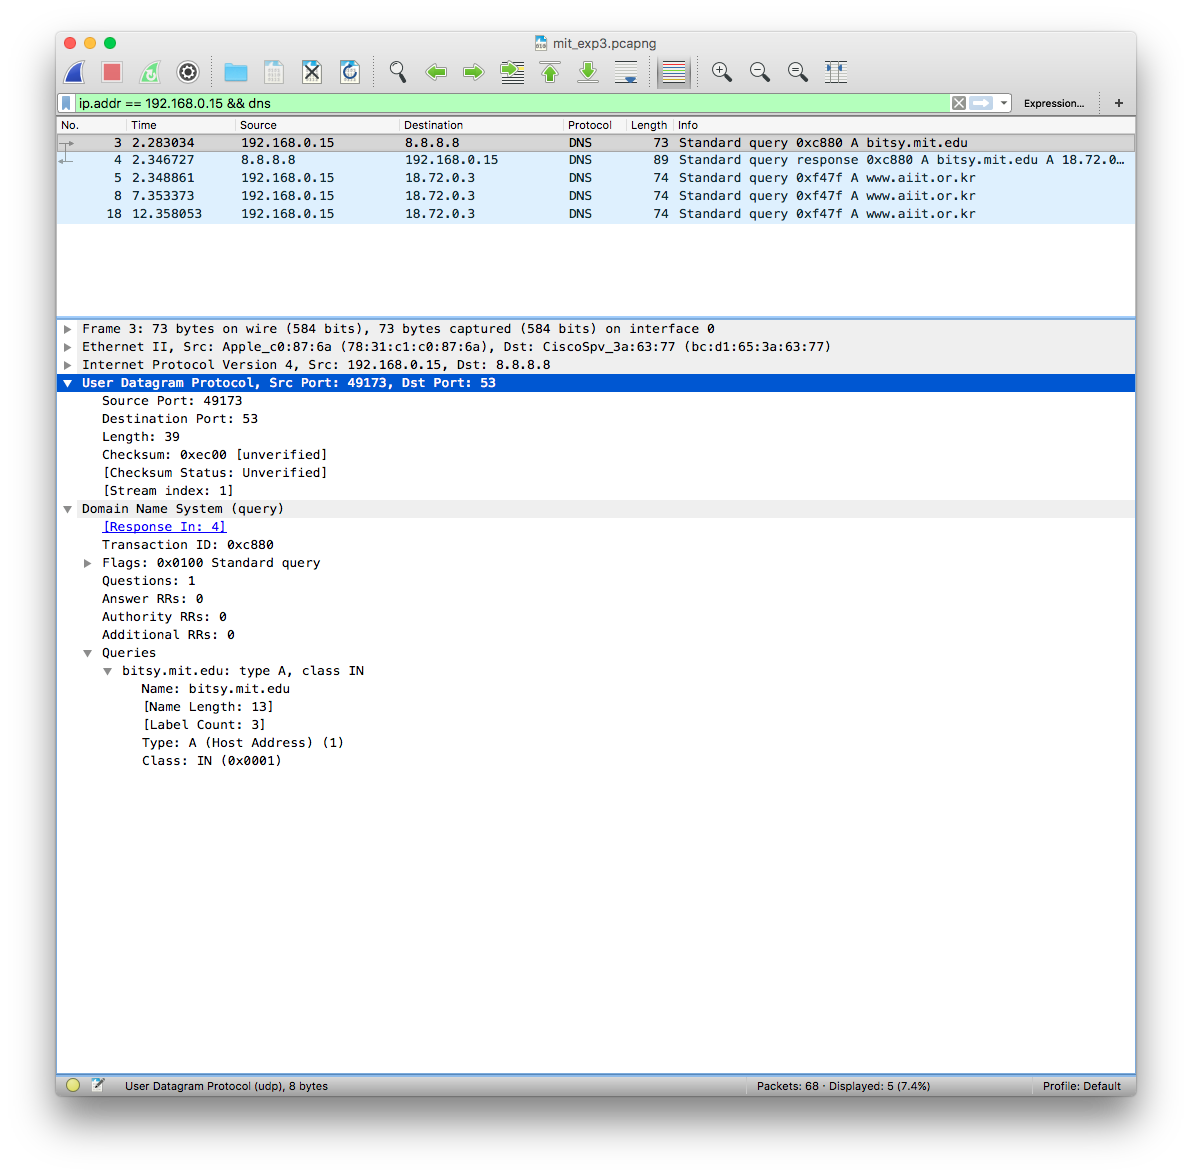
\includegraphics[width=460px]{14}
		\label{fig:14}
		\end{figure}
		
		\begin{figure}[H]
		\centering
		\caption{nslookup www.aiit.or.kr bitsy.mit.edu (DNS Response)}
		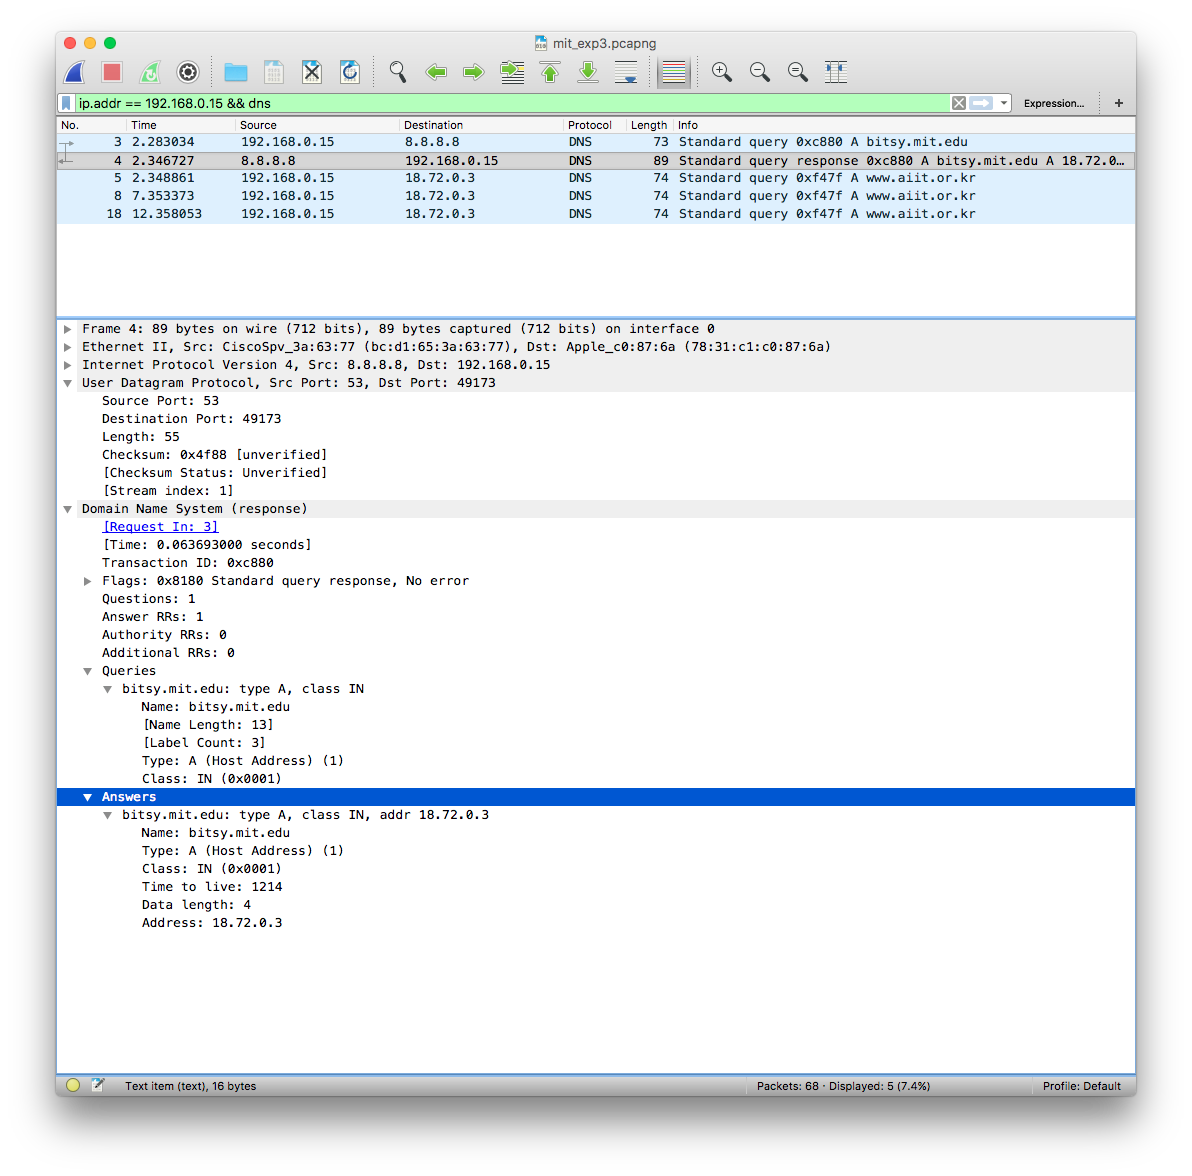
\includegraphics[width=460px]{15}
		\label{fig:15}
		\end{figure}
		
\pagebreak

	\item
		\textit{To what IP address is the DNS query message sent? Is this the IP address of your default local DNS server? If not, what does the IP address correspond to?}
		\par The DNS query message is sent to 8.8.8.8, which is the IP address of one of the local DNS servers.
		
	\item
		\textit{Examine the DNS query message. What “Type” of DNS query is it? Does the query message contain any “answers”?}
		\par Type A. It doesn't contain any answers.
		
	\item
		\textit{Examine the DNS response message. How many “answers” are provided? What does each of these answers contain?}
		\par Only one answer is provided. The answer contains the following information: name of the host, type, class, TTL, data length and IP address.
		
	\item
		\textit{Provide a screenshot.}
		\par Figures \ref{fig:14} and \ref{fig:15}.

\end{itemize}

\end{document}
